
\begin{frame}
\frametitle{Resultados de Regresión Agrupada}

  Regresión Agrupada: Hacemos regresión lineal sobre todos los datos, independientemente de su origen.

  \begin{enumerate}
    \item Para $\fwentrainment{AB}^{(1)}$ no hubo casi resultados significativos
    \item Para $\fwentrainment{AB}^{(2)}$ hubo resultados significativos, pero pocos
  \end{enumerate}

  Para analizar mejor los resultados y eliminar las variables no medidas, efectuamos un análisis de Efectos Fijos.
\end{frame}

\begin{frame}
\frametitle{Regresión Lineal con Efectos Fijos}

  \begin{columns}
    \column{0.40\textwidth}
    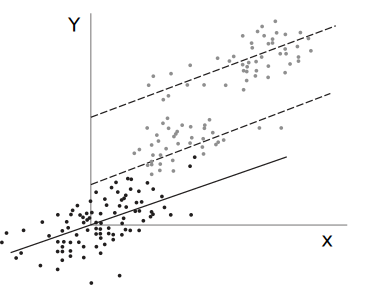
\includegraphics[width=\textwidth]{images/fixed_effects_example.pdf}
    \column{0.60\textwidth}
    \begin{itemize}
      \item Modelo agrupado: niega la posibilidad de heterogeneidad por cada sujeto
      \item Modelo efectos fijos: heterogeneidad no observada constante en el tiempo para cada sujeto.
      \item Varias formas equivalentes de calcularlo: Dummy Variable, Within Group.
      \item En nuestro caso: un sujeto es un hablante dentro de una sesión particular.
    \end{itemize}
  \end{columns}


\end{frame}
